\documentclass[10pt,fleqn]{article} % Default font size and left-justified equations
\usepackage[%
    pdftitle={Informatique : Introduction à l'algorithmique},
    pdfauthor={Xavier Pessoles}]{hyperref}

%%%%%%%%%%%%%%%%%%%%%%%%%%%%%%%%%%%%%%%%%
% Original author:
% Mathias Legrand (legrand.mathias@gmail.com) with modifications by:
% Vel (vel@latextemplates.com)
% License:
% CC BY-NC-SA 3.0 (http://creativecommons.org/licenses/by-nc-sa/3.0/)
%%%%%%%%%%%%%%%%%%%%%%%%%%%%%%%%%%%%%%%%%

%----------------------------------------------------------------------------------------
%	VARIOUS REQUIRED PACKAGES AND CONFIGURATIONS
%----------------------------------------------------------------------------------------

% Définition des booleéns
\newif\iffiche
\newif\ifprof
\newif\iftd
\newif\ifcours


\usepackage[top=2.5cm,bottom=2cm,left=2cm,right=2cm,headsep=40pt,a4paper]{geometry} % Page margins

\usepackage{graphicx} % Required for including pictures
\graphicspath{{images/}} % Specifies the directory where pictures are stored

\usepackage{lipsum} % Inserts dummy text

\usepackage{tikz} % Required for drawing custom shapes

\usepackage[french]{babel} % English language/hyphenation
\frenchbsetup{StandardLists=true} % Pour éviter la collision babel enumitem pour les listes

\usepackage{enumitem} % Customize lists
\setlist{nolistsep} % Reduce spacing between bullet points and numbered lists

\usepackage{booktabs} % Required for nicer horizontal rules in tables

\usepackage{colortbl} % Couleur dans les tableaux

\usepackage{xcolor} % Required for specifying colors by name
%\definecolor{ocre}{RGB}{243,102,25} % Define the orange color used for highlighting throughout the book
\definecolor{ocre}{RGB}{49,133,156} % Couleur ''bleue''
\definecolor{violetf}{RGB}{112,48,160} % Couleur ''violet''
\usepackage{enumitem}
\usepackage{pifont} % Pour les dinglist
\usepackage{multicol}
\usepackage{array} % Centrage vertical dans les tableaux

%----------------------------------------------------------------------------------------
%	FONTS
%----------------------------------------------------------------------------------------

\usepackage{avant} % Use the Avantgarde font for headings
%\usepackage{times} % Use the Times font for headings
%\usepackage{mathptmx} % Use the Adobe Times Roman as the default text font together with math symbols from the Sym­bol, Chancery and Com­puter Modern fonts
\usepackage[adobe-utopia]{mathdesign}
\usepackage{microtype} % Slightly tweak font spacing for aesthetics
\usepackage[utf8]{inputenc} % Required for including letters with accents
\usepackage[T1]{fontenc} % Use 8-bit encoding that has 256 glyphs

%----------------------------------------------------------------------------------------
%	BIBLIOGRAPHY AND INDEX
%----------------------------------------------------------------------------------------

\usepackage[style=alphabetic,citestyle=numeric,sorting=nyt,sortcites=true,autopunct=true,babel=hyphen,hyperref=true,abbreviate=false,backref=true,backend=biber]{biblatex}
\addbibresource{bibliography.bib} % BibTeX bibliography file
\defbibheading{bibempty}{}

\usepackage{calc} % For simpler calculation - used for spacing the index letter headings correctly
\usepackage{makeidx} % Required to make an index
\makeindex % Tells LaTeX to create the files required for indexing

%----------------------------------------------------------------------------------------
%	MAIN TABLE OF CONTENTS
%----------------------------------------------------------------------------------------

\usepackage{titletoc} % Required for manipulating the table of contents

\setcounter{tocdepth}{2}     % Dans la table des matieres
\setcounter{secnumdepth}{2}

\contentsmargin{0cm} % Removes the default margin

% Part text styling
\titlecontents{part}[0cm]
{\addvspace{20pt}\centering\large\bfseries}
{}
{}
{}

% Chapter text styling
\titlecontents{chapter}[1.25cm] % Indentation
{\addvspace{12pt}\large\sffamily\bfseries} % Spacing and font options for chapters
{\color{ocre!60}\contentslabel[\Large\thecontentslabel]{1.25cm}\color{ocre}} % Chapter number
{\color{ocre}}  
{\color{ocre!60}\normalsize\;\titlerule*[.5pc]{.}\;\thecontentspage} % Page number

% Section text styling
\titlecontents{section}[1.25cm] % Indentation
{\addvspace{3pt}\sffamily\bfseries} % Spacing and font options for sections
{\color{ocre!60}\contentslabel[\thecontentslabel]{1.25cm} \color{ocre}} % Section number
{\color{ocre}}
{\hfill\color{ocre!60}\thecontentspage} % Page number
[]

% Subsection text styling
\titlecontents{subsection}[1.25cm] % Indentation
{\addvspace{1pt}\sffamily\small} % Spacing and font options for subsections
{\contentslabel[\thecontentslabel]{1.25cm}} % Subsection number
{}
{\ \titlerule*[.5pc]{.}\;\thecontentspage} % Page number
[]


% Subsection text styling
\titlecontents{subsubsection}[1.25cm] % Indentation
{\addvspace{1pt}\sffamily\small} % Spacing and font options for subsections
{\contentslabel[\thecontentslabel]{1.25cm}} % Subsection number
{}
{\ \titlerule*[.5pc]{.}\;\thecontentspage} % Page number
[]

% List of figures
\titlecontents{figure}[0em]
{\addvspace{-5pt}\sffamily}
{\thecontentslabel\hspace*{1em}}
{}
{\ \titlerule*[.5pc]{.}\;\thecontentspage}
[]

% List of tables
\titlecontents{table}[0em]
{\addvspace{-5pt}\sffamily}
{\thecontentslabel\hspace*{1em}}
{}
{\ \titlerule*[.5pc]{.}\;\thecontentspage}
[]

%----------------------------------------------------------------------------------------
%	MINI TABLE OF CONTENTS IN PART HEADS
%----------------------------------------------------------------------------------------

% Chapter text styling
\titlecontents{lchapter}[0em] % Indenting
{\addvspace{15pt}\large\sffamily\bfseries} % Spacing and font options for chapters
{\color{ocre}\contentslabel[\Large\thecontentslabel]{1.25cm}\color{ocre}} % Chapter number
{}  
{\color{ocre}\normalsize\sffamily\bfseries\;\titlerule*[.5pc]{.}\;\thecontentspage} % Page number

% Section text styling
\titlecontents{lsection}[0em] % Indenting
{\sffamily\small} % Spacing and font options for sections
{\contentslabel[\thecontentslabel]{1.25cm}} % Section number
{}
{}

% Subsection text styling
\titlecontents{lsubsection}[.5em] % Indentation
{\normalfont\footnotesize\sffamily} % Font settings
{}
{}
{}

%----------------------------------------------------------------------------------------
%	PAGE HEADERS
%----------------------------------------------------------------------------------------

\usepackage{fancyhdr} % Required for header and footer configuration



\pagestyle{fancy}
 \renewcommand{\headrulewidth}{0pt}
 \fancyhead{}
 \fancyhead[L]{%
 \noindent\begin{minipage}[c]{2.6cm}%
 
\includegraphics[width=2cm]{png/logo_lycee.png}%
 \end{minipage}}

\fancyhead[C]{\rule{8cm}{.5pt}}

 \fancyhead[R]{%
 \noindent\begin{minipage}[c]{3cm}
 \begin{flushright}
 \footnotesize{\textit{\textsf{\xxtete}}}%
 \end{flushright}
 \end{minipage}
}


\fancyfoot[C]{\rule{12cm}{.5pt}}
\renewcommand{\footrulewidth}{0.2pt}
\fancyfoot[C]{\footnotesize{\bfseries \thepage}}
\fancyfoot[L]{ 
\begin{minipage}[c]{.2\linewidth}
\noindent\footnotesize{{\xxauteur}}
\end{minipage}}


\fancyfoot[R]{\footnotesize{\xxpied}
\ifthenelse{\isodd{\value{page}}}{
\begin{tikzpicture}[overlay]
\node[shape=rectangle, 
      rounded corners = .25 cm,
	  draw= ocre,
	  line width=2pt, 
	  fill = ocre!10,
	  minimum width  = 2.5cm,
	  minimum height = 3cm,] at (\xxposongletx,\xxposonglety) {};
\node at (\xxposonglettext,\xxposonglety) {\rotatebox{90}{\textbf{\large\color{ocre}{\xxonglet}}}};
%{};
\end{tikzpicture}}{}
}
%
%
%
% Removes the header from odd empty pages at the end of chapters
\makeatletter
\renewcommand{\cleardoublepage}{
\clearpage\ifodd\c@page\else
\hbox{}
\vspace*{\fill}
\thispagestyle{empty}
\newpage
\fi}

\fancypagestyle{plain}{%
\fancyhf{} % vide l’en-tête et le pied~de~page.
%\fancyfoot[C]{\bfseries \thepage} % numéro de la page en cours en gras
% et centré en pied~de~page.
\fancyfoot[R]{\footnotesize{\xxpied}}
\fancyfoot[C]{\rule{12cm}{.5pt}}
\renewcommand{\footrulewidth}{0.2pt}
\fancyfoot[C]{\footnotesize{\bfseries \thepage}}
\fancyfoot[L]{ 
\begin{minipage}[c]{.2\linewidth}
\noindent\footnotesize{{\xxauteur}}
\end{minipage}}}



%----------------------------------------------------------------------------------------
%	THEOREM STYLES
%----------------------------------------------------------------------------------------

% Conflit avec la police adobe
%\usepackage{amsmath,amsfonts,amssymb,amsthm} % For math equations, theorems, symbols, etc
\usepackage{amsmath,amsthm}

\newcommand{\intoo}[2]{\mathopen{]}#1\,;#2\mathclose{[}}
\newcommand{\ud}{\mathop{\mathrm{{}d}}\mathopen{}}
\newcommand{\intff}[2]{\mathopen{[}#1\,;#2\mathclose{]}}
%\newtheorem{notation}{Notation}[chapter]
\newtheorem{notation}{Notation}[section]

% Boxed/framed environments
\newtheoremstyle{ocrenumbox}% % Theorem style name
{0pt}% Space above
{0pt}% Space below
{\normalfont}% % Body font
{}% Indent amount
{\small\bf\sffamily\color{ocre}}% % Theorem head font
{\;}% Punctuation after theorem head
{0.25em}% Space after theorem head
{\small\sffamily\color{ocre}\thmname{#1}\nobreakspace\thmnumber%{\@ifnotempty{#1}{}\@upn{#2}}% Theorem text (e.g. Theorem 2.1)
\thmnote{\nobreakspace\the\thm@notefont\sffamily\bfseries\color{black}---\nobreakspace#3.}} % Optional theorem note
\renewcommand{\qedsymbol}{$\blacksquare$}% Optional qed square


% Boite pour les corriges
\newtheoremstyle{correctionbox}% % Theorem style name
{0pt}% Space above
{0pt}% Space below
{\normalfont}% % Body font
{}% Indent amount
{\small\bf\sffamily\color{violet}}% % Theorem head font
{\;}% Punctuation after theorem head
{0.25em}% Space after theorem head
{\small\sffamily\color{ocre}\thmname{#1}\nobreakspace\thmnumber%{\@ifnotempty{#1}{}\@upn{#2}}% Theorem text (e.g. Theorem 2.1)
\thmnote{\nobreakspace\the\thm@notefont\sffamily\bfseries\color{black}---\nobreakspace#3.}} % Optional theorem note
\renewcommand{\qedsymbol}{$\blacksquare$}% Optional qed square



\newtheoremstyle{blacknumex}% Theorem style name
{5pt}% Space above
{5pt}% Space below
{\normalfont}% Body font
{} % Indent amount
{\small\bf\sffamily}% Theorem head font
{\;}% Punctuation after theorem head
{0.25em}% Space after theorem head
{\small\sffamily{\tiny\ensuremath{\blacksquare}}\nobreakspace\thmname{#1}\nobreakspace\thmnumber%{\@ifnotempty{#1}{}\@upn{#2}}% Theorem text (e.g. Theorem 2.1)
\thmnote{\nobreakspace\the\thm@notefont\sffamily\bfseries---\nobreakspace#3.}}% Optional theorem note

\newtheoremstyle{blacknumbox} % Theorem style name
{0pt}% Space above
{0pt}% Space below
{\normalfont}% Body font
{}% Indent amount
{\small\bf\sffamily}% Theorem head font
{\;}% Punctuation after theorem head
{0.25em}% Space after theorem head
{\small\sffamily\thmname{#1}\nobreakspace 
\thmnote{\nobreakspace\the\thm@notefont\sffamily\bfseries---\nobreakspace#3.}}% Optional theorem note

% Non-boxed/non-framed environments
\newtheoremstyle{ocrenum}% % Theorem style name
{5pt}% Space above
{5pt}% Space below
{\normalfont}% % Body font
{}% Indent amount
{\small\bf\sffamily\color{ocre}}% % Theorem head font
{\;}% Punctuation after theorem head
{0.25em}% Space after theorem head
{\small\sffamily\color{ocre}\thmname{#1}\nobreakspace%\thmnumber{\@ifnotempty{#1}{}\@upn{#2}}% Theorem text (e.g. Theorem 2.1)
\thmnote{\nobreakspace\the\thm@notefont\sffamily\bfseries\color{black}---\nobreakspace#3.}} % Optional theorem note
\renewcommand{\qedsymbol}{$\blacksquare$}% Optional qed square
\makeatother

% Environnement pour les titres de parties
\newtheoremstyle{partiebox} 
{0pt}% Space above
{0pt}% Space below
{\normalfont}% Body font
{}% Indent amount
{\small\bf\sffamily}% Theorem head font
{\;}% Punctuation after theorem head
{0.25em}% Space after theorem head




% Defines the theorem text style for each type of theorem to one of the three styles above
\newcounter{dummy} 
\numberwithin{dummy}{section}
\theoremstyle{ocrenumbox}
%\newtheorem{theoremeT}[dummy]{Théorème}
\newtheorem{theoremeT}[dummy]{Théorème}
\newtheorem{resultatT}[dummy]{Résultat}
\newtheorem{savoirT}[dummy]{Savoir}
\newtheorem{methodeT}[dummy]{Méthode}
\newtheorem{objectifT}[dummy]{Objectif}
%\newtheorem{problem}{Problem}[chapter]
\newtheorem{problem}{Problem}[section]
%\newtheorem{exerciseT}{Exercise}[chapter]
\newtheorem{exerciseT}{Exercice}[section]

\theoremstyle{blacknumex}
%\newtheorem{exampleT}{Example}[chapter]
\newtheorem{exempleT}{Exemple}[section]
\newtheorem{termT}{Terminal\\}[section]
\newtheorem{pyT}{Python\\}[section]
\newtheorem{sciT}{Scilab\\}[section]
\newtheorem{pseudoT}{Pseudo Code\\}[section]
\newtheorem{sqlT}{SQL\\}[section]

\theoremstyle{blacknumbox}
%\newtheorem{vocabulary}{Vocabulary}[chapter]
\newtheorem{vocabulary}{Vocabulaire}[section]
%\newtheorem{definitionT}{Definition}[section]
\newtheorem{definitionT}{Définition}[section]
\newtheorem{demoT}{Démonstration}[section]
\newtheorem{corollaryT}[dummy]{Corollaire}
\newtheorem{hypoT}{Hypothèse(s)}

\theoremstyle{ocrenum}
\newtheorem{proposition}[dummy]{Proposition}

\theoremstyle{partiebox}
\newtheorem{titrepartieT}[]{}
\newtheorem{titrechapitreT}[]{}

\theoremstyle{correctionbox}
\newtheorem{correctionT}[dummy]{\color{violet}{Correction}}

%----------------------------------------------------------------------------------------
%	DEFINITION OF COLORED BOXES
%----------------------------------------------------------------------------------------

\RequirePackage[framemethod=tikz]{mdframed} % Required for creating the theorem, definition, exercise and corollary boxes

% Theorem box
\newmdenv[skipabove=7pt,
skipbelow=7pt,
backgroundcolor=ocre!10,
linecolor=ocre,
innerleftmargin=5pt,
innerrightmargin=5pt,
innertopmargin=5pt,
leftmargin=0cm,
rightmargin=0cm,
innerbottommargin=5pt]{tBox}


% Correction
\newmdenv[skipabove=7pt,
skipbelow=7pt,
backgroundcolor=violet!10,
linecolor=violet,
innerleftmargin=5pt,
innerrightmargin=5pt,
innertopmargin=5pt,
leftmargin=0cm,
rightmargin=0cm,
innerbottommargin=5pt]{coBox}


% Exercise box	  
\newmdenv[skipabove=7pt,
skipbelow=7pt,
rightline=false,
leftline=true,
topline=false,
bottomline=false,
backgroundcolor=ocre!10,
linecolor=ocre,
innerleftmargin=5pt,
innerrightmargin=5pt,
innertopmargin=5pt,
innerbottommargin=5pt,
leftmargin=0cm,
rightmargin=0cm,
linewidth=4pt]{eBox}	

% Definition box
\newmdenv[skipabove=7pt,
skipbelow=7pt,
rightline=false,
leftline=true,
topline=false,
bottomline=false,
backgroundcolor=ocre!10,
linecolor=ocre,
innerleftmargin=5pt,
innerrightmargin=5pt,
innertopmargin=0pt,
leftmargin=0cm,
rightmargin=0cm,
linewidth=4pt,
innerbottommargin=0pt]{dBox}	

% Demonstration box
\newmdenv[skipabove=7pt,
skipbelow=7pt,
rightline=false,
leftline=true,
topline=false,
bottomline=false,
%backgroundcolor=ocre!10,
linecolor=ocre,
innerleftmargin=5pt,
innerrightmargin=5pt,
innertopmargin=0pt,
leftmargin=0cm,
rightmargin=0cm,
linewidth=4pt,
innerbottommargin=0pt]{demoBox}	

% Corollary box
\newmdenv[skipabove=7pt,
skipbelow=7pt,
rightline=false,
leftline=true,
topline=false,
bottomline=false,
linecolor=gray,
backgroundcolor=black!5,
innerleftmargin=5pt,
innerrightmargin=5pt,
innertopmargin=5pt,
leftmargin=0cm,
rightmargin=0cm,
linewidth=4pt,
innerbottommargin=5pt]{cBox}


% Hypothèses
\newmdenv[skipabove=7pt,
skipbelow=7pt,
rightline=false,
leftline=true,
topline=false,
bottomline=false,
linecolor=gray,
backgroundcolor=black!5,
innerleftmargin=5pt,
innerrightmargin=5pt,
innertopmargin=5pt,
leftmargin=0cm,
rightmargin=0cm,
linewidth=4pt,
innerbottommargin=5pt]{hyBox}


% Boite pour le titre de la partie (pBox)
\newmdenv[skipabove=7pt,
skipbelow=7pt,
rightline=true,
leftline=false,
topline=false,
bottomline=false,
linecolor=ocre,
backgroundcolor=none,
innerleftmargin=5pt,
innerrightmargin=5pt,
innertopmargin=5pt,
leftmargin=0cm,
rightmargin=0cm,
linewidth=4pt,
innerbottommargin=5pt]{pBox}

% Boite pour le titre du chapitre (chBox)
\newmdenv[skipabove=7pt,
skipbelow=7pt,
rightline=false,
leftline=true,
topline=false,
bottomline=false,
linecolor=ocre,
%backgroundcolor=black!5,
innerleftmargin=5pt,
innerrightmargin=5pt,
innertopmargin=5pt,
leftmargin=0cm,
rightmargin=0cm,
linewidth=4pt,
innerbottommargin=5pt]{chBox}


% Boite pour les exemples
\newmdenv[skipabove=7pt,
skipbelow=7pt,
rightline=false,
leftline=true,
topline=false,
bottomline=false,
linecolor=gray,
backgroundcolor=white,
innerleftmargin=5pt,
innerrightmargin=5pt,
innertopmargin=5pt,
leftmargin=0cm,
rightmargin=0cm,
linewidth=4pt,
innerbottommargin=5pt]{exBox}

% Boite pour le terminal
\newmdenv[skipabove=7pt,
skipbelow=7pt,
rightline=false,
leftline=true,
topline=false,
bottomline=false,
linecolor=gray,
backgroundcolor=white,
innerleftmargin=5pt,
innerrightmargin=5pt,
innertopmargin=5pt,
leftmargin=0cm,
rightmargin=0cm,
linewidth=4pt,
innerbottommargin=5pt]{termBox}


% Boite pour Python
\newmdenv[skipabove=7pt,
skipbelow=7pt,
rightline=false,
leftline=true,
topline=false,
bottomline=false,
linecolor=gray,
backgroundcolor=white,
innerleftmargin=5pt,
innerrightmargin=5pt,
innertopmargin=5pt,
leftmargin=0cm,
rightmargin=0cm,
linewidth=4pt,
innerbottommargin=5pt]{pyBox}

% Boite pour scilab
\newmdenv[skipabove=7pt,
skipbelow=7pt,
rightline=false,
leftline=true,
topline=false,
bottomline=false,
linecolor=gray,
backgroundcolor=white,
innerleftmargin=5pt,
innerrightmargin=5pt,
innertopmargin=5pt,
leftmargin=0cm,
rightmargin=0cm,
linewidth=4pt,
innerbottommargin=5pt]{sciBox}


% Boite pour pseudo
\newmdenv[skipabove=7pt,
skipbelow=7pt,
rightline=false,
leftline=true,
topline=false,
bottomline=false,
linecolor=gray,
backgroundcolor=white,
innerleftmargin=5pt,
innerrightmargin=5pt,
innertopmargin=5pt,
leftmargin=0cm,
rightmargin=0cm,
linewidth=4pt,
innerbottommargin=5pt]{pseudoBox}

% Boite pour pseudo
\newmdenv[skipabove=7pt,
skipbelow=7pt,
rightline=false,
leftline=true,
topline=false,
bottomline=false,
linecolor=gray,
backgroundcolor=white,
innerleftmargin=5pt,
innerrightmargin=5pt,
innertopmargin=5pt,
leftmargin=0cm,
rightmargin=0cm,
linewidth=4pt,
innerbottommargin=5pt]{sqlBox}


% Creates an environment for each type of theorem and assigns it a theorem text style from the "Theorem Styles" section above and a colored box from above
\newenvironment{theorem}{\begin{tBox}\begin{theoremeT}}{\end{theoremeT}\end{tBox}}
\newenvironment{resultat}{\begin{tBox}\begin{resultatT}}{\end{resultatT}\end{tBox}}
\newenvironment{methode}{\begin{tBox}\begin{methodeT}}{\end{methodeT}\end{tBox}}
\newenvironment{savoir}{\begin{tBox}\begin{savoirT}}{\end{savoirT}\end{tBox}}
\newenvironment{obj}{\begin{tBox}\begin{objectifT}}{\end{objectifT}\end{tBox}}
\newenvironment{corrige}{\begin{coBox}\begin{correctionT}}{\end{correctionT}\end{coBox}}
\newenvironment{exercise}{\begin{eBox}\begin{exerciseT}}{\hfill{\color{ocre}\tiny\ensuremath{\blacksquare}}\end{exerciseT}\end{eBox}}				  
\newenvironment{exercice}{\begin{eBox}\begin{exerciseT}}{\hfill{\color{ocre}\tiny\ensuremath{\blacksquare}}\end{exerciseT}\end{eBox}}				  

\newenvironment{definition}{\begin{dBox}\begin{definitionT}}{\end{definitionT}\end{dBox}}	
\newenvironment{defi}{\begin{dBox}\begin{definitionT}}{\end{definitionT}\end{dBox}}	
\newenvironment{demo}{\begin{demoBox}\begin{demoT}}{\end{demoT}\end{demoBox}}	
%\newenvironment{exemple}{\begin{exempleT}}{\hfill{\tiny\ensuremath{\blacksquare}}\end{exempleT}}		
\newenvironment{corollary}{\begin{cBox}\begin{corollaryT}}{\end{corollaryT}\end{cBox}}
\newenvironment{hypo}{\begin{hyBox}\begin{hypoT}}{\end{hypoT}\end{hyBox}}	\newenvironment{exemple}{\begin{exBox}\begin{exempleT}}{\hfill{\tiny\ensuremath{\blacksquare}}\end{exempleT}\end{exBox}}	
\newenvironment{titrepartie}{\begin{pBox}\begin{titrepartieT}}{\end{titrepartieT}\end{pBox}}	
\newenvironment{titrechapitre}{\begin{chBox}\begin{titrechapitreT}}{\end{titrechapitreT}\end{chBox}}	

\newenvironment{term}{ \begin{termBox}\begin{termT}}{\end{termT}\end{termBox}}
\newenvironment{py}{ \begin{pyBox}\begin{pyT}}{\end{pyT}\end{pyBox}}
\newenvironment{sci}{ \begin{sciBox}\begin{sciT}}{\end{sciT}\end{sciBox}}
\newenvironment{pseudo}{ \begin{pseudoBox}\begin{pseudoT}}{\end{pseudoT}\end{pseudoBox}}
\newenvironment{envsql}{ \begin{sqlBox}\begin{sqlT}}{\end{sqlT}\end{sqlBox}}


%----------------------------------------------------------------------------------------
%	REMARK ENVIRONMENT
%----------------------------------------------------------------------------------------

\newenvironment{remark}{\par\vspace{10pt}\small % Vertical white space above the remark and smaller font size
\begin{list}{}{
\leftmargin=35pt % Indentation on the left
\rightmargin=25pt}\item\ignorespaces % Indentation on the right
\makebox[-2.5pt]{\begin{tikzpicture}[overlay]
\node[draw=ocre!60,line width=1pt,circle,fill=ocre!25,font=\sffamily\bfseries,inner sep=2pt,outer sep=0pt] at (-15pt,0pt){\textcolor{ocre}{R}};\end{tikzpicture}} % Orange R in a circle
\advance\baselineskip -1pt}{\end{list}\vskip5pt} % Tighter line spacing and white space after remark

\newenvironment{rem}{\par\vspace{10pt}\small % Vertical white space above the remark and smaller font size
\begin{list}{}{
\leftmargin=35pt % Indentation on the left
\rightmargin=25pt}\item\ignorespaces % Indentation on the right
\makebox[-2.5pt]{\begin{tikzpicture}[overlay]
\node[draw=ocre!60,line width=1pt,circle,fill=ocre!25,font=\sffamily\bfseries,inner sep=2pt,outer sep=0pt] at (-15pt,0pt){\textcolor{ocre}{R}};\end{tikzpicture}} % Orange R in a circle
\advance\baselineskip -1pt}{\end{list}\vskip5pt} % Tighter line spacing and white space after remark


\newenvironment{warn}{\par\vspace{10pt}\small % Vertical white space above the remark and smaller font size
\begin{list}{}{
\leftmargin=35pt % Indentation on the left
\rightmargin=25pt}\item\ignorespaces % Indentation on the right
\makebox[-2.5pt]{\begin{tikzpicture}[overlay]
\node[draw=red!60,line width=1pt,circle,fill=red!25,font=\sffamily\bfseries,inner sep=2pt,outer sep=0pt] at (-15pt,0pt){\textcolor{black}{!}};\end{tikzpicture}} % Point d'exclamation dans un cercle
\advance\baselineskip -1pt}{\end{list}\vskip5pt} % Tighter line spacing and white space after remark


%----------------------------------------------------------------------------------------
%	SECTION NUMBERING IN THE MARGIN
%----------------------------------------------------------------------------------------
\setcounter{secnumdepth}{3}
\setcounter{tocdepth}{2}



\makeatletter
\renewcommand{\@seccntformat}[1]{\llap{\textcolor{ocre}{\csname the#1\endcsname}\hspace{1em}}}                    
\renewcommand{\section}{\@startsection{section}{1}{\z@}
{-4ex \@plus -1ex \@minus -.4ex}
{1ex \@plus.2ex }
{\normalfont\large\sffamily\bfseries}}
\renewcommand{\subsection}{\@startsection {subsection}{2}{\z@}
{-3ex \@plus -0.1ex \@minus -.4ex}
{0.5ex \@plus.2ex }
{\normalfont\sffamily\bfseries}}
\renewcommand{\subsubsection}{\@startsection {subsubsection}{3}{\z@}
{-2ex \@plus -0.1ex \@minus -.2ex}
{.2ex \@plus.2ex }
{\normalfont\small\sffamily\bfseries}}                        
\renewcommand\paragraph{\@startsection{paragraph}{4}{\z@}
{-2ex \@plus-.2ex \@minus .2ex}
{.1ex}
{\normalfont\small\sffamily\bfseries}}

%----------------------------------------------------------------------------------------
%	PART HEADINGS
%----------------------------------------------------------------------------------------


%----------------------------------------------------------------------------------------
%	CHAPTER HEADINGS
%----------------------------------------------------------------------------------------

% \newcommand{\thechapterimage}{}%
% \newcommand{\chapterimage}[1]{\renewcommand{\thechapterimage}{#1}}%
% \def\@makechapterhead#1{%
% {\parindent \z@ \raggedright \normalfont
% \ifnum \c@secnumdepth >\m@ne
% \if@mainmatter
% \begin{tikzpicture}[remember picture,overlay]
% \node at (current page.north west)
% {\begin{tikzpicture}[remember picture,overlay]
% \node[anchor=north west,inner sep=0pt] at (0,0) {\includegraphics[width=\paperwidth]{\thechapterimage}};
% \draw[anchor=west] (\Gm@lmargin,-9cm) node [line width=2pt,rounded corners=15pt,draw=ocre,fill=white,fill opacity=0.5,inner sep=15pt]{\strut\makebox[22cm]{}};
% \draw[anchor=west] (\Gm@lmargin+.3cm,-9cm) node {\huge\sffamily\bfseries\color{black}\thechapter. #1\strut};
% \end{tikzpicture}};
% \end{tikzpicture}
% \else
% \begin{tikzpicture}[remember picture,overlay]
% \node at (current page.north west)
% {\begin{tikzpicture}[remember picture,overlay]
% \node[anchor=north west,inner sep=0pt] at (0,0) {\includegraphics[width=\paperwidth]{\thechapterimage}};
% \draw[anchor=west] (\Gm@lmargin,-9cm) node [line width=2pt,rounded corners=15pt,draw=ocre,fill=white,fill opacity=0.5,inner sep=15pt]{\strut\makebox[22cm]{}};
% \draw[anchor=west] (\Gm@lmargin+.3cm,-9cm) node {\huge\sffamily\bfseries\color{black}#1\strut};
% \end{tikzpicture}};
% \end{tikzpicture}
% \fi\fi\par\vspace*{270\p@}}}

%-------------------------------------------

\def\@makeschapterhead#1{%
\begin{tikzpicture}[remember picture,overlay]
\node at (current page.north west)
{\begin{tikzpicture}[remember picture,overlay]
\node[anchor=north west,inner sep=0pt] at (0,0) {\includegraphics[width=\paperwidth]{\thechapterimage}};
\draw[anchor=west] (\Gm@lmargin,-9cm) node [line width=2pt,rounded corners=15pt,draw=ocre,fill=white,fill opacity=0.5,inner sep=15pt]{\strut\makebox[22cm]{}};
\draw[anchor=west] (\Gm@lmargin+.3cm,-9cm) node {\huge\sffamily\bfseries\color{black}#1\strut};
\end{tikzpicture}};
\end{tikzpicture}
\par\vspace*{270\p@}}
\makeatother

%----------------------------------------------------------------------------------------
%	HYPERLINKS IN THE DOCUMENTS
%----------------------------------------------------------------------------------------


\hypersetup{hidelinks,backref=true,pagebackref=true,hyperindex=true,colorlinks=false,breaklinks=true,urlcolor= ocre,bookmarks=true,bookmarksopen=false,pdftitle={Title},pdfauthor={Author}}
\usepackage{bookmark}
\bookmarksetup{
open,
numbered,
addtohook={%
\ifnum\bookmarkget{level}=0 % chapter
\bookmarksetup{bold}%
\fi
\ifnum\bookmarkget{level}=-1 % part
\bookmarksetup{color=ocre,bold}%
\fi
}
}

%----------------------------------------------------------------------------------------
%	
%----------------------------------------------------------------------------------------

\newcommand{\thechapterimage}{}%
\newcommand{\chapterimage}[1]{\renewcommand{\thechapterimage}{#1}}%
\def\@makechapterhead#1{%
{\parindent \z@ \raggedright \normalfont
\begin{tikzpicture}[remember picture,overlay]
\node at (current page.north west)
{\begin{tikzpicture}[remember picture,overlay]
\node[anchor=north west,inner sep=0pt] at (0,0) {\includegraphics[width=\paperwidth]{\thechapterimage}};
%\draw[anchor=west] (\Gm@lmargin,-9cm) node [line width=2pt,rounded corners=15pt,draw=ocre,fill=white,fill opacity=0.5,inner sep=15pt]{\strut\makebox[22cm]{}};
%\draw[anchor=west] (\Gm@lmargin+.3cm,-9cm) node {\huge\sffamily\bfseries\color{black}\thechapter. #1\strut};
\end{tikzpicture}};
\end{tikzpicture}
\par\vspace*{270\p@}
}}




\makeatletter             
\renewcommand{\subparagraph}{\@startsection{subparagraph}{5}{\z@}%
                                    {-2ex \@plus-.2ex \@minus .2ex}%
                                    {0ex}%               
{\normalfont\bfseries Question \hspace{.7cm} }}
\makeatother
\renewcommand{\thesubparagraph}{\arabic{subparagraph}} 
\makeatletter


%%%% Environnement pour inclure du code
\usepackage{textcomp}
\usepackage[french]{algorithm2e}
\usepackage{listings}
\lstloadlanguages{R}   % pour regler les pb d accent utf8 dans les codes
\lstset{language=R} % pour regler les pb d accent utf8 dans les codes
\renewcommand{\lstlistlistingname}{Listings}
\renewcommand{\lstlistingname}{Listing}

\SetKwBlock{Fonction}{Début Fonction}{Fin Fonction}
\SetKwComment{Comment}{start}{end}

\definecolor{Bleu}{rgb}{0.1,0.1,1.0}
\definecolor{Noir}{rgb}{0,0,0}
\definecolor{Grau}{rgb}{0.5,0.5,0.5}
\definecolor{DunkelGrau}{rgb}{0.15,0.15,0.15}
\definecolor{Hellbraun}{rgb}{0.5,0.25,0.0}
\definecolor{Magenta}{rgb}{1.0,0.0,1.0}
\definecolor{Gris}{gray}{0.5}
\definecolor{Vert}{rgb}{0,0.5,0}
\definecolor{SourceHintergrund}{rgb}{1,1.0,0.95}


\lstnewenvironment{python}[1][]{
\lstset{
%escapeinside={\%*}{*)},
inputencoding=utf8,   % pour regler les pb d accent utf8 dans les codes
extendedchars=true,   % pour regler les pb d accent utf8 dans les codes
language=python,
basicstyle=\sffamily\footnotesize, 	
stringstyle=\color{red}, 
showstringspaces=false, 
alsoletter={1234567890},
otherkeywords={\ , \}, \{},
keywordstyle=\color{blue},
emph={access,and,break,class,continue,def,del,elif ,else,
except,exec,finally,for,from,global,if,import,in,i s,
lambda,not,or,pass,print,raise,return,try,while},
emphstyle=\color{black}\bfseries,
emph={[2]True, False, None, self},
emphstyle=[2]\color{black},
emph={[3]from, import, as},
emphstyle=[3]\color{blue},
upquote=true,
columns=flexible, % pour empecher d'avoir un espacement mono
morecomment=[s]{"""}{"""},
commentstyle=\color{Hellbraun}\slshape, 
%emph={[4]1, 2, 3, 4, 5, 6, 7, 8, 9, 0},
emphstyle=[4]\color{blue},
literate=*{:}{{\textcolor{blue}:}}{1}
{=}{{\textcolor{blue}=}}{1}
{-}{{\textcolor{blue}-}}{1}
{+}{{\textcolor{blue}+}}{1}
{*}{{\textcolor{blue}*}}{1}
{!}{{\textcolor{blue}!}}{1}
{(}{{\textcolor{blue}(}}{1}
{)}{{\textcolor{blue})}}{1}
{[}{{\textcolor{blue}[}}{1}
{]}{{\textcolor{blue}]}}{1}
{<}{{\textcolor{blue}<}}{1}
{>}{{\textcolor{blue}>}}{1}
{COMPLETER}{{\textcolor{red}COMPLETER}}{1},
literate=%
            {é}{{\'{e}}}1
            {è}{{\`{e}}}1
            {ê}{{\^{e}}}1
            {ë}{{\¨{e}}}1
            {û}{{\^{u}}}1
            {ù}{{\`{u}}}1
            {â}{{\^{a}}}1
            {à}{{\`{a}}}1
            {î}{{\^{i}}}1
            {ç}{{\c{c}}}1
            {Ç}{{\c{C}}}1
            {É}{{\'{E}}}1
            {Ê}{{\^{E}}}1
            {À}{{\`{A}}}1
            {Â}{{\^{A}}}1
            {Î}{{\^{I}}}1, % pour regler les pb d accent utf8 dans les codes
%framexleftmargin=1mm, framextopmargin=1mm, frame=shadowbox, rulesepcolor=\color{blue},#1
%backgroundcolor=\color{SourceHintergrund}, 
%framexleftmargin=1mm, framexrightmargin=1mm, framextopmargin=1mm, frame=single, framerule=1pt, rulecolor=\color{black},#1
}}{}



\lstnewenvironment{scilab}[1][]{
\lstset{
language=scilab,
basicstyle=\sffamily\footnotesize, 	
stringstyle=\color{red}, 
showstringspaces=false, 
alsoletter={1234567890},
otherkeywords={\ , \}, \{},
keywordstyle=\color{blue},
emph={access,and,break,class,continue,def,del,elif ,else,
except,exec,finally,for,from,global,if,import,in,i s,
lambda,not,or,pass,print,raise,return,try,while,Debut},
emphstyle=\color{black}\bfseries,
emph={[2]True, False, None, self},
emphstyle=[2]\color{black},
emph={[3]from, import, as},
emphstyle=[3]\color{blue},
upquote=true,
columns=flexible, % pour empecher d'avoir un espacement mono
morecomment=[s]{"""}{"""},
commentstyle=\color{Hellbraun}\slshape, 
%emph={[4]1, 2, 3, 4, 5, 6, 7, 8, 9, 0},
emphstyle=[4]\color{blue},
literate=*{:}{{\textcolor{blue}:}}{1}
{=}{{\textcolor{blue}=}}{1}
{-}{{\textcolor{blue}-}}{1}
{+}{{\textcolor{blue}+}}{1}
{*}{{\textcolor{blue}*}}{1}
{!}{{\textcolor{blue}!}}{1}
{(}{{\textcolor{blue}(}}{1}
{)}{{\textcolor{blue})}}{1}
{[}{{\textcolor{blue}[}}{1}
{]}{{\textcolor{blue}]}}{1}
{<}{{\textcolor{blue}<}}{1}
{>}{{\textcolor{blue}>}}{1},
%framexleftmargin=1mm, framextopmargin=1mm, frame=shadowbox, rulesepcolor=\color{blue},#1
%backgroundcolor=\color{SourceHintergrund}, 
%framexleftmargin=1mm, framexrightmargin=1mm, framextopmargin=1mm, frame=single, framerule=1pt, rulecolor=\color{black},#1
}}{}


\lstdefinestyle{stylepython}{%
escapeinside={\%*}{*)},
inputencoding=utf8,   % pour regler les pb d accent utf8 dans les codes
extendedchars=true,   % pour regler les pb d accent utf8 dans les codes
language=python,
basicstyle=\sffamily\footnotesize, 	
stringstyle=\color{red}, 
showstringspaces=false, 
alsoletter={1234567890},
otherkeywords={\ , \}, \{},
keywordstyle=\color{blue},
emph={access,and,break,class,continue,def,del,elif ,else,
except,exec,finally,for,from,global,if,import,in,i s,
lambda,not,or,pass,print,raise,return,try,while},
emphstyle=\color{black}\bfseries,
emph={[2]True, False, None, self},
emphstyle=[2]\color{green},
emph={[3]from, import, as},
emphstyle=[3]\color{blue},
upquote=true,
columns=flexible, % pour empecher d'avoir un espacement mono
morecomment=[s]{"""}{"""},
commentstyle=\color{Hellbraun}\slshape, 
%emph={[4]1, 2, 3, 4, 5, 6, 7, 8, 9, 0},
emphstyle=[4]\color{blue},
literate=*{:}{{\textcolor{blue}:}}{1}
{=}{{\textcolor{blue}=}}{1}
{-}{{\textcolor{blue}-}}{1}
{+}{{\textcolor{blue}+}}{1}
{*}{{\textcolor{blue}*}}{1}
{!}{{\textcolor{blue}!}}{1}
{(}{{\textcolor{blue}(}}{1}
{)}{{\textcolor{blue})}}{1}
{[}{{\textcolor{blue}[}}{1}
{]}{{\textcolor{blue}]}}{1}
{<}{{\textcolor{blue}<}}{1}
{>}{{\textcolor{blue}>}}{1}
{COMPLETER}{{\textcolor{red}COMPLETER}}{1},
literate=%
            {é}{{\'{e}}}1
            {è}{{\`{e}}}1
            {ê}{{\^{e}}}1
            {ë}{{\¨{e}}}1
            {û}{{\^{u}}}1
            {ù}{{\`{u}}}1
            {â}{{\^{a}}}1
            {à}{{\`{a}}}1
            {î}{{\^{i}}}1
            {ç}{{\c{c}}}1
            {Ç}{{\c{C}}}1
            {É}{{\'{E}}}1
            {Ê}{{\^{E}}}1
            {À}{{\`{A}}}1
            {Â}{{\^{A}}}1
            {Î}{{\^{I}}}1,
%numbers=left,                    % where to put the line-numbers; possible values are (none, left, right)
%numbersep=5pt,                   % how far the line-numbers are from the code
%numberstyle=\tiny\color{mygray}, % the style that is used for the line-numbers
}



\lstnewenvironment{termi}[1][]{
\lstset{
language=scilab,
basicstyle=\sffamily\footnotesize, 	
stringstyle=\color{red}, 
showstringspaces=false, 
alsoletter={1234567890},
otherkeywords={\ , \}, \{},
keywordstyle=\color{blue},
emph={access,and,break,class,continue,def,del,elif ,else,
except,exec,finally,for,from,global,if,import,in,i s,
lambda,not,or,pass,print,raise,return,try,while,Debut},
emphstyle=\color{black}\bfseries,
emph={[2]True, False, None, self},
emphstyle=[2]\color{green},
emph={[3]from, import, as},
emphstyle=[3]\color{blue},
upquote=true,
columns=flexible, % pour empecher d'avoir un espacement mono
morecomment=[s]{"""}{"""},
commentstyle=\color{Hellbraun}\slshape, 
%emph={[4]1, 2, 3, 4, 5, 6, 7, 8, 9, 0},
emphstyle=[4]\color{blue},
literate=*{:}{{\textcolor{blue}:}}{1}
{=}{{\textcolor{blue}=}}{1}
{-}{{\textcolor{blue}-}}{1}
{+}{{\textcolor{blue}+}}{1}
{*}{{\textcolor{blue}*}}{1}
{!}{{\textcolor{blue}!}}{1}
{(}{{\textcolor{blue}(}}{1}
{)}{{\textcolor{blue})}}{1}
{[}{{\textcolor{blue}[}}{1}
{]}{{\textcolor{blue}]}}{1}
{<}{{\textcolor{blue}<}}{1}
{>}{{\textcolor{blue}>}}{1},
%framexleftmargin=1mm, framextopmargin=1mm, frame=shadowbox, rulesepcolor=\color{blue},#1
%backgroundcolor=\color{SourceHintergrund}, 
%framexleftmargin=1mm, framexrightmargin=1mm, framextopmargin=1mm, frame=single, framerule=1pt, rulecolor=\color{black},#1
}}{}


\lstnewenvironment{sql}[1][]{
\lstset{
%escapeinside={\%*}{*)},
%inputencoding=utf8,   % pour regler les pb d accent utf8 dans les codes
%extendedchars=true,   % pour regler les pb d accent utf8 dans les codes
language=sql,
basicstyle=\sffamily\footnotesize, 	
stringstyle=\color{red}, 
showstringspaces=false, 
alsoletter={1234567890},
otherkeywords={\ , \}, \{},
keywordstyle=\color{blue},
emph={access,and,break,class,continue,def,del,elif ,else,
except,exec,finally,for,from,global,if,import,in,i s,
lambda,not,or,pass,print,raise,return,try,while},
emphstyle=\color{black}\bfseries,
emph={[2]True, False, None, self},
emphstyle=[2]\color{black},
emph={[3]from, import, as},
emphstyle=[3]\color{blue},
upquote=true,
columns=flexible, % pour empecher d'avoir un espacement mono
morecomment=[s]{"""}{"""},
commentstyle=\color{Hellbraun}\slshape, 
%emph={[4]1, 2, 3, 4, 5, 6, 7, 8, 9, 0},
emphstyle=[4]\color{blue},
literate=*{:}{{\textcolor{blue}:}}{1}
{=}{{\textcolor{blue}=}}{1}
{-}{{\textcolor{blue}-}}{1}
{+}{{\textcolor{blue}+}}{1}
{*}{{\textcolor{blue}*}}{1}
{!}{{\textcolor{blue}!}}{1}
{(}{{\textcolor{blue}(}}{1}
{)}{{\textcolor{blue})}}{1}
{[}{{\textcolor{blue}[}}{1}
{]}{{\textcolor{blue}]}}{1}
{<}{{\textcolor{blue}<}}{1}
{>}{{\textcolor{blue}>}}{1}
{COMPLETER}{{\textcolor{red}COMPLETER}}{1},
literate=%
            {é}{{\'{e}}}1
            {è}{{\`{e}}}1
            {ê}{{\^{e}}}1
            {ë}{{\¨{e}}}1
            {û}{{\^{u}}}1
            {ù}{{\`{u}}}1
            {â}{{\^{a}}}1
            {à}{{\`{a}}}1
            {î}{{\^{i}}}1
            {ç}{{\c{c}}}1
            {Ç}{{\c{C}}}1
            {É}{{\'{E}}}1
            {Ê}{{\^{E}}}1
            {À}{{\`{A}}}1
            {Â}{{\^{A}}}1
            {Î}{{\^{I}}}1, % pour regler les pb d accent utf8 dans les codes
%framexleftmargin=1mm, framextopmargin=1mm, frame=shadowbox, rulesepcolor=\color{blue},#1
%backgroundcolor=\color{SourceHintergrund}, 
%framexleftmargin=1mm, framexrightmargin=1mm, framextopmargin=1mm, frame=single, framerule=1pt, rulecolor=\color{black},#1
}}{}



%%%%%%%%%%%%
% Définition des vecteurs 
%%%%%%%%%%%%
 \newcommand{\vect}[1]{\overrightarrow{#1}}
\newcommand{\axe}[2]{\left(#1,\vect{#2}\right)}

\newcommand{\rep}[1]{\mathcal{R}_{#1}}
\newcommand{\vx}[1]{\vect{x_{#1}}}
\newcommand{\vy}[1]{\vect{y_{#1}}}
\newcommand{\vz}[1]{\vect{z_{#1}}}

%%%%%%%%%%%%
% Définition des torseurs 
%%%%%%%%%%%%

 \newcommand{\torseur}[1]{%
\left\{{#1}\right\}
}

\newcommand{\torseurcin}[3]{%
\left\{\mathcal{#1} \left(#2/#3 \right) \right\}
}

\newcommand{\torseurstat}[3]{%
\left\{\mathcal{#1} \left(#2\rightarrow #3 \right) \right\}
}

 \newcommand{\torseurc}[8]{%
%\left\{#1 \right\}=
\left\{
{#1}
\right\}
 = 
\left\{%
\begin{array}{cc}%
{#2} & {#5}\\%
{#3} & {#6}\\%
{#4} & {#7}\\%
\end{array}%
\right\}_{#8}%
}

 \newcommand{\torseurcol}[7]{
\left\{%
\begin{array}{cc}%
{#1} & {#4}\\%
{#2} & {#5}\\%
{#3} & {#6}\\%
\end{array}%
\right\}_{#7}%
}

 \newcommand{\torseurl}[3]{%
%\left\{\mathcal{#1}\right\}_{#2}=%
\left\{%
\begin{array}{l}%
{#1} \\%
{#2} %
\end{array}%
\right\}_{#3}%
}

 \newcommand{\vectv}[3]{%
\vect{V\left( {#1} \in {#2}/{#3}\right)}
}


\newcommand{\vectf}[2]{%
\vect{R\left( {#1} \rightarrow {#2}\right)}
}

\newcommand{\vectm}[3]{%
\vect{\mathcal{M}\left( {#1}, {#2} \rightarrow {#3}\right)}
}


 \newcommand{\vectg}[3]{%
\vect{\Gamma \left( {#1} \in {#2}/{#3}\right)}
}

 \newcommand{\vecto}[2]{%
\vect{\Omega\left( {#1}/{#2}\right)}
}
% }$$\left\{\mathcal{#1} \right\}_{#2} =%
% \left\{%
% \begin{array}{c}%
%  #3 \\%
%  #4 %
% \end{array}%
% \right\}_{#5}}

%\fichetrue
\fichefalse

%\proftrue
\proffalse

%\tdtrue
\tdfalse

\courstrue
%\coursfalse

% -------------------------------------
% Déclaration des titres
% -------------------------------------

\def\discipline{Informatique}
\def\xxtete{Informatique}

\def\classe{PTSI}
\def\xxnumpartie{Partie 2}
\def\xxpartie{Algorithmique \& Programmation}

\def\xxnumchapitre{Chapitre 4}
\def\xxchapitre{\hspace{.12cm} Introduction à la complexité}

\def\xxposongletx{2}
\def\xxposonglettext{1.45}
\def\xxposonglety{22}%19

\def\xxonglet{Part. 2 -- Ch. 4}

\def\xxactivite{Cours}
\def\xxauteur{\textsl{Xavier Pessoles}}

\def\xxcompetences{%
\textsl{%
\textbf{Savoirs et compétences :}
\begin{itemize}[label=\ding{112},font=\color{ocre}] 
\item s'interroger sur l'efficacité algorithmique temporelle.
\end{itemize}
}}

\def\xxfigures{
}%figues de la page de garde

\def\xxpied{%
Partie 2 -- Algorithmique \& Programmation \\
Ch 4 : Introduction à la complexité -- \xxactivite%
}

%---------------------------------------------------------------------------
\begin{document}
\chapterimage{png/Fond_ALG}
\pagestyle{empty}


%%%%%%%% PAGE DE GARDE COURS
\ifcours
\begin{tikzpicture}[remember picture,overlay]
\node at (current page.north west)
{\begin{tikzpicture}[remember picture,overlay]
\node[anchor=north west,inner sep=0pt] at (0,0) {\includegraphics[width=\paperwidth]{\thechapterimage}};
\draw[anchor=west] (-2cm,-8cm) node [line width=2pt,rounded corners=15pt,draw=ocre,fill=white,fill opacity=0.6,inner sep=40pt]{\strut\makebox[22cm]{}};
\draw[anchor=west] (1cm,-8cm) node {\huge\sffamily\bfseries\color{black} %
\begin{minipage}{1cm}
\rotatebox{90}{\LARGE\sffamily\textsc{\color{ocre}\textbf{\xxnumpartie}}}
\end{minipage} \hfill
\begin{minipage}[c]{14cm}
\begin{titrepartie}
\begin{flushright}
\renewcommand{\baselinestretch}{1.1} 
\Large\sffamily\textsc{\textbf{\xxpartie}}
\renewcommand{\baselinestretch}{1} 
\end{flushright}
\end{titrepartie}
\end{minipage} \hfill
\begin{minipage}[c]{3.5cm}
{\large\sffamily\textsc{\textbf{\color{ocre} \discipline}}}
\end{minipage} 
 };
\end{tikzpicture}};
\end{tikzpicture}


\begin{tikzpicture}[overlay]
\node[shape=rectangle, 
      rounded corners = .25 cm,
	  draw= ocre,
	  line width=2pt, 
	  fill = ocre!10,
	  minimum width  = 2.5cm,
	  minimum height = 3cm,] at (18cm,0) {};
\node at (17.7cm,0) {\rotatebox{90}{\textbf{\Large\color{ocre}{\classe}}}};
%{};
\end{tikzpicture}

\vspace{3.5cm}

\begin{tikzpicture}[remember picture,overlay]
\draw[anchor=west] (-2cm,-6cm) node {\huge\sffamily\bfseries\color{black} %
\begin{minipage}{2cm}
\begin{center}
\LARGE\sffamily\textsc{\color{ocre}\textbf{\xxactivite}}
\end{center}
\end{minipage} \hfill
\begin{minipage}[c]{15cm}
\begin{titrechapitre}
\renewcommand{\baselinestretch}{1.1} 
\Large\sffamily\textsc{\textbf{\xxnumchapitre}}

\Large\sffamily\textsc{\textbf{\xxchapitre}}
\vspace{.5cm}

\renewcommand{\baselinestretch}{1} 
\normalsize\normalfont
\xxcompetences
\end{titrechapitre}
\end{minipage}  };
\end{tikzpicture}
\vfill

\begin{flushright}
\begin{minipage}[c]{.3\linewidth}
\begin{center}
\xxfigures
\end{center}
\end{minipage}\hfill
\begin{minipage}[c]{.6\linewidth}
\startcontents
\printcontents{}{1}{}
\end{minipage}
\end{flushright}

\begin{tikzpicture}[remember picture,overlay]
\draw[anchor=west] (4.5cm,-.7cm) node {
\begin{minipage}[c]{.2\linewidth}
\begin{flushright}

\includegraphics[width=2cm]{png/logoCC}
\end{flushright}
\end{minipage}
\begin{minipage}[c]{.2\linewidth}
\textsl{\xxauteur} \\
\textsl{\classe}
\end{minipage}
 };
\end{tikzpicture}
\newpage
\pagestyle{fancy}

\newpage
\pagestyle{fancy}

\else
\fi


%%%%%%%% PAGE DE GARDE TD
\iftd
%\begin{tikzpicture}[remember picture,overlay]
%\node at (current page.north west)
%{\begin{tikzpicture}[remember picture,overlay]
%\draw[anchor=west] (-2cm,-3.25cm) node [line width=2pt,rounded corners=15pt,draw=ocre,fill=white,fill opacity=0.6,inner sep=40pt]{\strut\makebox[22cm]{}};
%\draw[anchor=west] (1cm,-3.25cm) node {\huge\sffamily\bfseries\color{black} %
%\begin{minipage}{1cm}
%\rotatebox{90}{\LARGE\sffamily\textsc{\color{ocre}\textbf{\xxnumpartie}}}
%\end{minipage} \hfill
%\begin{minipage}[c]{13.5cm}
%\begin{titrepartie}
%\begin{flushright}
%\renewcommand{\baselinestretch}{1.1} 
%\Large\sffamily\textsc{\textbf{\xxpartie}}
%\renewcommand{\baselinestretch}{1} 
%\end{flushright}
%\end{titrepartie}
%\end{minipage} \hfill
%\begin{minipage}[c]{3.5cm}
%{\large\sffamily\textsc{\textbf{\color{ocre} \discipline}}}
%\end{minipage} 
% };
%\end{tikzpicture}};
%\end{tikzpicture}

%%%%%%%%%% PAGE DE GARDE TD %%%%%%%%%%%%%%%
%\begin{tikzpicture}[overlay]
%\node[shape=rectangle, 
%      rounded corners = .25 cm,
%	  draw= ocre,
%	  line width=2pt, 
%	  fill = ocre!10,
%	  minimum width  = 2.5cm,
%	  minimum height = 2.5cm,] at (18.5cm,0) {};
%\node at (17.7cm,0) {\rotatebox{90}{\textbf{\Large\color{ocre}{\classe}}}};
%%{};
%\end{tikzpicture}

% PARTIE ET CHAPITRE
%\begin{tikzpicture}[remember picture,overlay]
%\draw[anchor=west] (-1cm,-2.1cm) node {\large\sffamily\bfseries\color{black} %
%\begin{minipage}[c]{15cm}
%\begin{flushleft}
%\xxnumchapitre \\
%\xxchapitre
%\end{flushleft}
%\end{minipage}  };
%\end{tikzpicture}

% Bandeau titre exo
\begin{tikzpicture}[remember picture,overlay]
\draw[anchor=west] (-2cm,-6cm) node {\huge\sffamily\bfseries\color{black} %
\begin{minipage}{5cm}
\begin{center}
\LARGE\sffamily\color{ocre}\textbf{\textsc{\xxactivite}}

\begin{center}
\xxfigures
\end{center}

\end{center}
\end{minipage} \hfill
\begin{minipage}[c]{12cm}
\begin{titrechapitre}
\renewcommand{\baselinestretch}{1.1} 
\large\sffamily\textbf{\textsc{\xxtitreexo}}

\small\sffamily{\textbf{\textit{\color{black!70}\xxsourceexo}}}
\vspace{.5cm}

\renewcommand{\baselinestretch}{1} 
\normalsize\normalfont
\xxcompetences
\end{titrechapitre}
\end{minipage}  };
\end{tikzpicture}

\else
\fi


%%%%%%%% PAGE DE GARDE FICHE
\iffiche
\begin{tikzpicture}[remember picture,overlay]
\node at (current page.north west)
{\begin{tikzpicture}[remember picture,overlay]
\draw[anchor=west] (-2cm,-3.25cm) node [line width=2pt,rounded corners=15pt,draw=ocre,fill=white,fill opacity=0.6,inner sep=40pt]{\strut\makebox[22cm]{}};
\draw[anchor=west] (1cm,-3.25cm) node {\huge\sffamily\bfseries\color{black} %
\begin{minipage}{1cm}
\rotatebox{90}{\LARGE\sffamily\textsc{\color{ocre}\textbf{\xxnumpartie}}}
\end{minipage} \hfill
\begin{minipage}[c]{14cm}
\begin{titrepartie}
\begin{flushright}
\renewcommand{\baselinestretch}{1.1} 
\large\sffamily\textsc{\textbf{\xxpartie} \\} 

\vspace{.2cm}

\normalsize\sffamily\textsc{\textbf{\xxnumchapitre -- \xxchapitre}}
\renewcommand{\baselinestretch}{1} 
\end{flushright}
\end{titrepartie}
\end{minipage} \hfill
\begin{minipage}[c]{3.5cm}
{\large\sffamily\textsc{\textbf{\color{ocre} \discipline}}}
\end{minipage} 
 };
\end{tikzpicture}};
\end{tikzpicture}


\begin{tikzpicture}[overlay]
\node[shape=rectangle, 
      rounded corners = .25 cm,
	  draw= ocre,
	  line width=2pt, 
	  fill = ocre!10,
	  minimum width  = 2.5cm,
%	  minimum height = 2.5cm,] at (18.5cm,0.5cm) {};
	  minimum height = 2.5cm,] at (18.5cm,0cm) {};
\node at (17.7cm,0) {\rotatebox{90}{\textsf{\textbf{\large\color{ocre}{\classe}}}}};
%{};
\end{tikzpicture}



\else
\fi



%---------------------------------------------------------------------------



\section{Mise en évidence du problème}

%\subsection{Premier exemple}
%On introduit les algorithmes de tri suivant : 
%\begin{py}
%\begin{python}
%#Tri par sélection
%def tri_selection(tab):
%    for i in range(0,len(tab)):
%        indice = i
%        for j in range(i+1,len(tab)):
%            if tab[j]<tab[indice]:
%               indice = j
%        tab[i],tab[indice]=tab[indice],tab[i]
%    return tab
%\end{python}
%\end{py}
%
%\begin{py}
%\begin{python}    
%#Tri par insertion
%def tri_insertion(tab):
%    for i in range(1,len(tab)):
%        a=tab[i] 
%        j=i-1    
%        while j>=0 and tab[j]>a:
%            tab[j+1]=tab[j]
%            j=j-1
%        tab[j+1]=a
%    return tab
%\end{python}
%\end{py}
%
%\begin{py}
%\begin{python}
%def shellSort(array):
%     "Shell sort using Shell's (original) gap sequence: n/2, n/4, ..., 1."
%     "http://en.wikibooks.org/wiki/Algorithm_Implementation/Sorting/Shell_sort#Python"
%     gap = len(array) // 2
%     # loop over the gaps
%     while gap > 0:
%         # do the insertion sort
%         for i in range(gap, len(array)):
%             val = array[i]
%             j = i
%             while j >= gap and array[j - gap] > val:
%                 array[j] = array[j - gap]
%                 j -= gap
%             array[j] = val
%         gap //= 2
%\end{python}
%\end{py}
%
%La figure ci-dessous montre le temps en secondes pour trier des tableaux de 1 à 1000 éléments en utilisant les méthodes de tri suivant : 
%\begin{itemize}
%\item tri par sélection;
%\item tri par insertion; 
%\item tri shell;
%\item méthode de tri utilisée par Python.
%\end{itemize}
%
%Le premier graphe montre le temps de calcul et le second une estimation du nombre d'opérations. 
%
%\begin{minipage}[c]{.48\linewidth}
%\begin{center}
%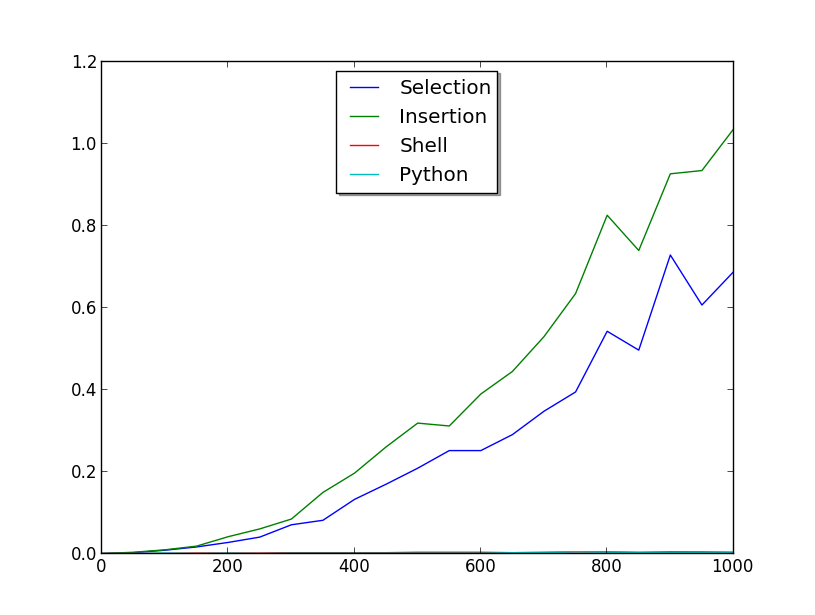
\includegraphics[width=.95\textwidth]{images/figure_1}
%\end{center}
%\end{minipage}\hfill
%\begin{minipage}[c]{.48\linewidth}
%\begin{center}
%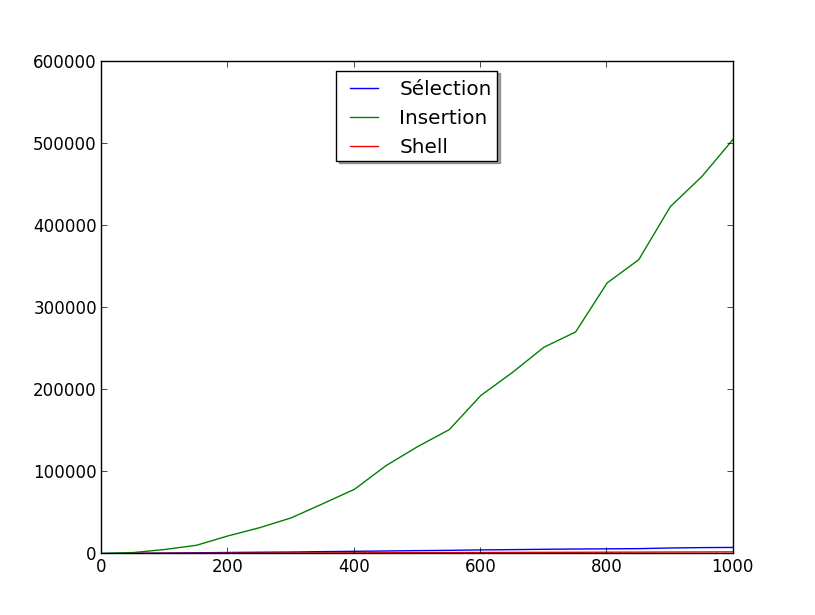
\includegraphics[width=.95\textwidth]{images/figure_2}
%\end{center}
%\end{minipage}

%\subsection{Deuxième exemple}
On prend l'exemple de la recherche d'un élément dans une liste : 



\begin{minipage}[c]{.49\linewidth}

\begin{pseudo}
\begin{center}
\begin{tabular}{p{.9\textwidth}}
\hline
\textbf{Algorithme :} Recherche d'un nombre dans une liste triée ou non \\
\hline
\textbf{Données :}
\begin{itemize}
\item \textsf{nb}, int : un entier 
\item \textsf{tab}, liste : une liste d'entiers triés ou non triés
\end{itemize}
\textbf{Résultat :} un booléen : \textsf{Vrai} si le nombre est dans la liste, \textsf{Faux} sinon. \\
\\
\textbf{is\_number\_in\_list}(\textsf{nb},\textsf{tab}) :\\
\hspace{.4cm}\textsf{l} $\leftarrow$ \textbf{longueur}(\textsf{tab}) \\
\hspace{.4cm}\textbf{Pour} \textsf{i} \textbf{allant de} 1 \textbf{à} \textsf{l} \textbf{faire} : \\
\hspace{.8cm} \textbf{Si}  \textsf{tab[i] = nb} \textbf{alors} :\\
\hspace{1.2cm}\textbf{Retourne} \textsf{Vrai} \\
\hspace{.8cm} \textbf{Fin Si} \\
\hspace{.4cm}\textbf{Fin Faire} \\
\hspace{.4cm}\textbf{Retourne} \textsf{Faux} \\
\textbf{Fin fonction} \\
\hline
\end{tabular}
\end{center}
\end{pseudo}
\end{minipage}\hfill
\begin{minipage}[c]{.49\linewidth}
\begin{py}
\begin{python}
def is_number_in_list(nb,tab):
    """Renvoie True si le nombre nb est dans la liste 
    de nombres tab
    Keyword arguments:
      * nb, int -- nombre entier
      * tab, list -- liste de nombres entiers    
    """
    for i in range(len(tab)):
        if tab[i]==nb:
            return True
    return False
\end{python}
\end{py}
\end{minipage}


\begin{exemple}
\`A partir de l'algorithme précédent, évaluer : 
\begin{itemize}
\item le nombre de tour de boucles dans le pire des cas;
\item le nombre de tour de boucles dans le meilleur des cas.
\end{itemize}
\end{exemple}

\begin{py}
\begin{python}
def is_number_in_list_dicho(nb,tab):
    """ 
    Recherche d'un nombre par dichotomie dans un tableau trié. 
    Renvoie l'index si le nombre nb est dans la liste de nombres tab.
    Renvoie None sinon.
    Keyword arguments:
    nb,int -- nombre entier
    tab,list -- liste de nombres entiers triés
    """
    g, d = 0, len(tab)-1
    while g <= d:
        m = (g + d) // 2
        if tab[m] == nb:
            return m
        if tab[m] < nb:
            g = m+1
        else:
            d = m-1
    return None
\end{python}
\end{py}



\begin{center}
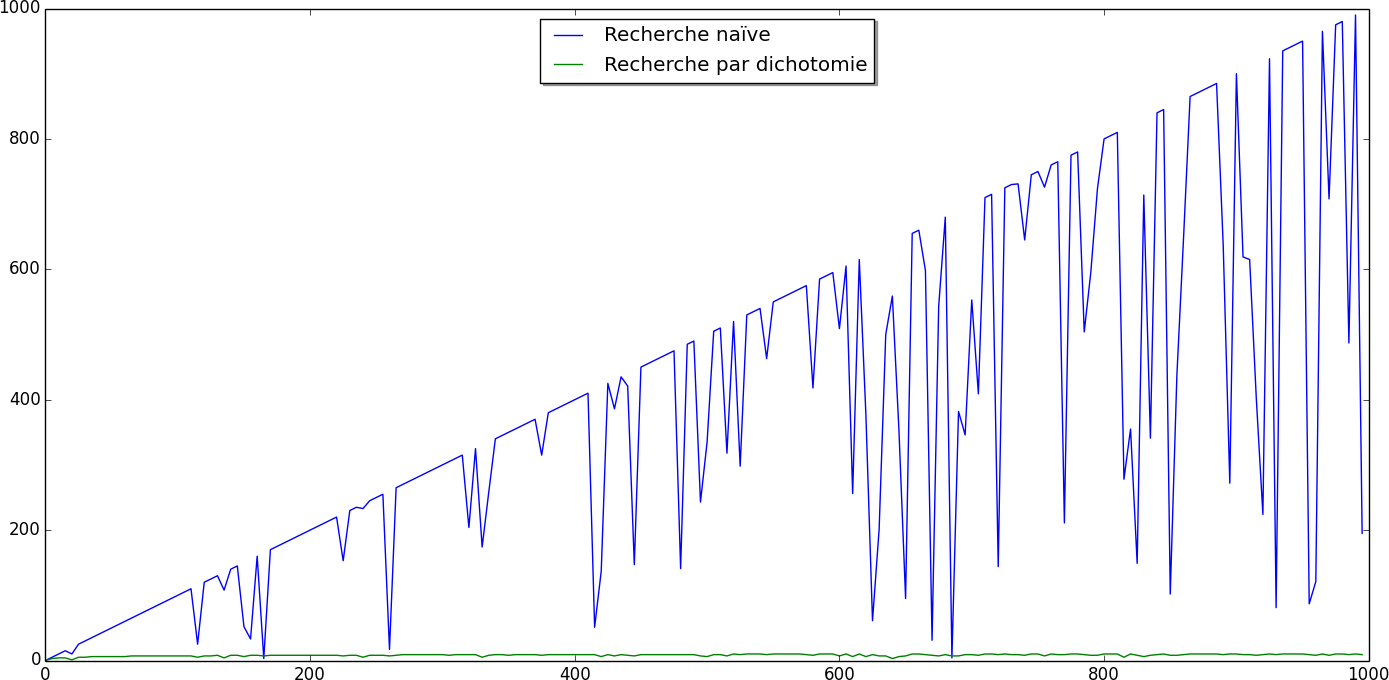
\includegraphics[width=.95\textwidth]{images/figure_5}

\textit{Évolution du nombre d'opérations pour rechercher un nombre dans une liste de 1 à 1000 nombres}
\end{center}



\section{Complexité des algorithmes}

\subsection{Présentation}
Il existe souvent plusieurs façons de programmer un algorithme. Si le nombre d'opérations à effectuer est peu important et les données d'entrée de l'algorithme sont de faibles tailles, le choix de la solution importe peu. En revanche, lorsque le nombre d'opérations et la taille des données d'entrée deviennent importants, deux paramètres deviennent déterminants : le temps d'exécution et l'occupation mémoire. 


\begin{defi}
\textbf{Complexité en temps}

La complexité en temps donne le nombre d'opérations effectuées lors de l'exécution d'un programme. On appelle $C_o$ le coût en temps d'une opération $o$.

\textbf{Complexité en mémoire (ou en espace)}

La complexité en mémoire donne le nombre d'emplacements mémoires occupés lors de l'exécution d'un programme.


\end{defi}

\begin{rem}

On distingue la complexité dans le pire des cas, la complexité dans le meilleure des cas, ou la complexité en moyenne. En effet, pour un même algorithme, suivant les données à manipuler, le résultat sera déterminé plus ou moins rapidement. 

Généralement, on s'intéresse au cas le plus défavorable à savoir, la complexité dans le pire des cas. 
\end{rem}

%\begin{resultat}
%Soit une suite de deux instructions ayant un coût respectif de $C_1$ et $C_2$. Le coût total de la suite d'opération est donc $C=C_1 + C_2$.
%
%Plus généralement, lorsqu'on réalise une itération, le coût total correspond à la somme des différents coûts. En notant $C_i$ le coût de la $i^{\text{ème}}$ suite d'instruction, le coût total de l'itération est donc :
%$$
%C = \sum\limits_{i=1}^{n}C_i
%$$
%\end{resultat}

\subsection{Coût temporel d'un algorithme et d'une opération}
\begin{minipage}[c]{.47\linewidth}
\begin{resultat}
On considère que le coût élémentaire $C_e$ correspond au coût d'une affectation, d'une comparaison ou de l'évaluation d'une opération arithmétique. 
\end{resultat}
\end{minipage}\hfill
\begin{minipage}[c]{.47\linewidth}
\begin{exemple}
Chacune de ces 3 opérations expressions ont le même coût temporel $C_e$:
\begin{py}
\begin{python}
>>> a=20
>>> a<=100
>>> a+a
\end{python}
\end{py}
\end{exemple}
\end{minipage}

\vspace{.5cm}

\begin{minipage}[c]{.47\linewidth}
\begin{resultat}
Pour une séquence de deux instructions de coûts respectifs $C_1$ et $C_2$, le coût total est de la séquence est de $C_1 + C_2$.
\end{resultat}
\end{minipage}\hfill
\begin{minipage}[c]{.47\linewidth}
\begin{exemple}
\begin{py}
\begin{python}
>>> a=20
>>> print(a)
\end{python}
\end{py}
Le coût temporel correspond à l'addition du coût élémentaire de l'affectation ajouté au coût de l'affichage.
\end{exemple}
\end{minipage}

\vspace{.5cm}

\begin{minipage}[c]{.47\linewidth}
\begin{resultat}
Le coût d'un test \textsf{if test : inst\_1 else : inst\_2 } est inférieur ou égal au maximum du coût de l'instruction 1 et du coût de l'instruction 2 additionné au coût du test (coût élémentaire). 
\end{resultat}
\end{minipage}\hfill
\begin{minipage}[c]{.47\linewidth}
\begin{exemple}
Soit le programme suivant (sans application réelle) :
\begin{py}
\begin{python}
>>>    if x<0 :
               x=x+1
               x=x+2
           else :
               x=x+1
\end{python}
\end{py}

La comparaison a un coût élémentaire $C_e$. Dans le <<~pire~>> des cas, on réalise deux additions et deux affectations. 
Le coût temporel total est est donc $C_e + 4C_e = 5C_e$.
\end{exemple}
\end{minipage}

\vspace{.5cm}

\begin{minipage}[c]{.47\linewidth}
\begin{resultat}
Le coût d'une boucle \textsf{for i in range(n) : inst}  est égal à : $n$ fois le coût de l'instruction \textsf{inst} si elle est indépendante de la valeur de $i$.
\end{resultat}
\end{minipage}\hfill
\begin{minipage}[c]{.47\linewidth}
\begin{exemple}

\begin{py}
\begin{python}
>>> for i in range(20) : print(i)
\end{python}
\end{py}
Si on note $C_p$ le coût de l'affichage, le coût total est de $20 C_p$.
\end{exemple}
\end{minipage}

\vspace{.5cm}

%\begin{minipage}[c]{.47\linewidth}
\begin{resultat}
Soit la boucle \textsf{while cond : inst}, la condition \textsf{cond} faisant intervenir un variant de boucle. Il est donc possible de connaître le nombre $n$ d'itérations de la boucle. 
Le coût de la boucle est donc égal à n fois le coût de l'instruction \textsf{inst}.
\end{resultat}
%\end{minipage}\hfill
%\begin{minipage}[c]{.47\linewidth}
%\begin{exemple}

%\begin{py}
%\begin{python}

%\end{python}
%\end{py}
%\end{exemple}
%\end{minipage}


\subsection{Exemple}

\begin{exemple}
\textit{Calcul de factorielle}

\begin{pseudo}
\begin{algorithm}[H]
\Fonction{
factorielle($n$):\\
\eSi{n=0}{
\Retour{1}
}{
$i\gets1$\\
$res\gets1$\\
\Tq{$i\leq n$}{
$res \gets res \cdot i$ \\
$i\gets i+1$}
\Retour{res}
}}
\end{algorithm}
\end{pseudo}

\textbf{Complexité en mémoire :} lors de l'exécution du programme, il sera nécessaire de stocker les variables suivantes : 
\begin{itemize}
\item $n$;
\item $res$;
\item $i$. 
\end{itemize}

\textbf{Complexité en temps :}
La première comparaison a un coût élémentaire $C_e$.

Pour $n=0$  le coût du retour est $C_r$.

Pour $n \neq 0$ :
\begin{itemize}
\item les deux affectations ont un coût respectif $C_e$;
\item la boucle tant que sera réalisée $n$ fois. Pour chaque itération, 
\begin{itemize}
\item la multiplication ainsi que l'affectation ont un chacun un coût $C_e$;
\item l'incrémentation et l'affectation ont chacun un coût $C_e$;
\end{itemize}
\item le coût du retour est $C_r$.
\end{itemize}
En conséquence, la complexité en temps s'élève à :
$$C_T(n) = C_e + \max\left( C_r;  C_e + C_e + n\left( 4C_e\right) + C_r\right)$$

Ainsi $C_T(n) = C_e (3 + 4n)  + C_r$ et $C_T(n)  \underset{+\infty}{\sim} 4C_e n$ lorsque $n$ tend vers l'infini. On parle d'une complexité algorithmique linéaire, notée $\mathcal{O}(n)$.

\end{exemple}



Il est fréquent que la complexité en temps soit améliorée au prix d'une augmentation de la complexité en espace, et vice-versa.
La complexité dépend notamment :
\begin{itemize}
\item de la puissance de la machine sur laquelle l'algorithme est exécuté;
\item du langage et compilateur / interpréteur utilisé pour coder l'algorithme;
\item du style du programmeur.
\end{itemize}


\begin{rem}
Le coût de la mémoire étant aujourd'hui relativement faible, on cherche en général à améliorer la complexité en temps plutôt que le complexité en mémoire. 
\end{rem}

\subsection{D'autres exemples}
\subsubsection{Recherche d'un maximum}
\begin{exemple}
\textit{Soit une liste de nombre entiers désordonnés. Comment déterminer le plus grand nombre de la liste ?}

Intuitivement, une solution est de parcourir la liste d'élément et de déterminer le plus grand élément par comparaisons successives.


\begin{pseudo}
\begin{algorithm}[H]
\KwData{$tab$ tableau de taille $n$}
$max  \leftarrow -\infty$\\
\For{$i=1$ \KwTo $n$}{
\If{$tab[i]>max$}{
$max  \leftarrow tab[i]$\\
}}
\end{algorithm}
\end{pseudo}

Dans ce cas, le coût temporel est :
$C_T(n) = C_e + n\left(2 C_e \right)$. Ici encore, la complexité de cet algorithme est linéaire car $C_T(n) \underset{+\infty}{\sim} 2 C_e n$.
\end{exemple}

\subsubsection{Tri d'une liste}

\begin{exemple}
\textbf{Algorithme naïf}

\textit{Soit une liste de nombre entiers désordonnés. Comment les trier par ordre croissant ?}

Une méthode dite naïve pourrait être la suivante : 
\begin{itemize}
\item trouver le plus petit élément du tableau. Notons $min$ son indice;
\item on permute alors le $min$\ieme élément avec le premier élément;
\item ...
\item on trouve le plus petit élément du tableau compris entre l'indice $i$ et $N$;
\item on permute alors le $min$\ieme élément avec le $i$\ieme élément.
\end{itemize}



\begin{pseudo}
\begin{algorithm}[H]
\KwData{$tab$ tableau d'entiers désordonnés de taille $n$}
\KwResult{$tab$ tableau d'entiers ordonnés}
\For{$i=1$ \KwTo $n-1$}{
$ min \leftarrow  i$\\
\For{$j=i+1$ \KwTo $n$}{
\If{$tab[j]<tab[min]$}{
$min  \leftarrow j$\\
}}
$tmp  \leftarrow tab[i]$ \\
$ tab[i] \leftarrow tab[min]$ \\
$ tab[min] \leftarrow tmp$ \\
}

\end{algorithm}
\end{pseudo}

Ici les bornes de la boucle imbriquée dépendent de l'indice $i$. Ainsi :
\begin{itemize}
\item au rang $1$, $C_1 = C_e + \left(n-1\right)\left( 2 C_e\right) + 3 C_e$;
\item au rang $2$, $C_2 = C_e + \left(n-2\right)\left( 2 C_e\right) + 3 C_e$;
\item au rang $i$, $C_i = C_e + \left(n-i)\right)\left( 2 C_e\right) + 3 C_e$.
\end{itemize}

Le coût temporel peut donc s'exprimer ainsi : 
\begin{eqnarray*}
C_T(n) &=& \sum\limits_{i=0}^{n} \left(Ce + (n-i)\left( 2 C_e\right) + 3 C_e \right) = C_e\sum\limits_{i=0}^{n} \left( 1+2n-2i + 3 \right) \\
&=&C_e\sum\limits_{i=0}^{n} \left( 4+2n-2i  \right) =  C_e \left( 4n+2n^2 -  2\dfrac{n(n+1)}{2}\right) = C_e\left( 3n+n^2\right)
%C_e \left( 5n + n^2  \right)
\end{eqnarray*}

Dans ce cas, $C_T(n)\sim C_e n^2$. On parle de complexité quadratique. Lorsque la taille du tableau double, le temps de calcul est multiplié par 4.

\end{exemple}

%\begin{rem}
%Il existe d'autres algorithmes de tris plus performant que l'algorithme présenté ci-dessus : 
%\begin{itemize}
%\item tri de shell (\textsf{shell sort});
%\item tri fusion (\textsf{merge sort});
%\item tri rapide (\textsf{quick sort})...
%\end{itemize}
%\end{rem}

\subsubsection{Diviser pour régner -- recherche dichotomique}
\begin{exemple}
\begin{py}
\begin{python}
def recherche_dichotomique(x, a):
    g, d = 0, len(a)-1
    while g <= d:
        m = (g + d) // 2
        if a[m] == x:
            return m
        elif a[m] < x:
            g = m+1
        else:
            d = m-1
    return None
\end{python}
\end{py}
On peut montrer que la suite $d-g$ décroit strictement (car $d$ décroit et $g$ croit).
Dans ce cas, la difficulté consiste en déterminer le nombre de fois que sera exécutée la boucle \textsf{while}. On note $C_w = C_e + \max\left(C_e + C_r ; 2 C_e + 2 C_e; 3 C_e + C_e \right) = C_e + \max\left(C_e + C_r ; 4 C_e  \right)$ le coût d'une itération de la boucle \textsf{while}.

Au cours de l'algorithme, on va devoir diviser en 2 la taille le tableau jusqu'à ce qu'on trouve (ou pas) l'élément recherché. On cherche donc combien de fois $m$ on peut diviser par 2 la taille du tableau $n$ :
$$
\dfrac{n}{2^m} \geq 1 \Longleftrightarrow n \geq 2^m \Longleftrightarrow \ln(n)\geq m \ln(2) $$
On parlera ici de complexité logarithmique.

%Au cours de l'algorithme, on va devoir diviser la quantité $g+d$ par 2 tant que $g$ est inférieur à $d$. On cherche donc $n$ tel que $g>d$. On considère que la borne $d$ est fixe. On note $p$ la taille du tableau donc $d=p \; \forall n\in\mathbb{N}$ et $g_0=1$.
%Exprimons la suite décrite par les valeurs de $g$ :
%\begin{eqnarray*}
%g_n &= &m_n + 1 = \dfrac{g_{n-1}+p}{2}+1 =\dfrac{1}{2}g_{n-1} + \dfrac{p}{2} + 1\\
%g_{n-1} &=& \dfrac{1}{2}g_{n-2} + \dfrac{p}{2} + 1 \\
%g_n &=& \dfrac{1}{2}\left( \dfrac{1}{2}g_{n-2} + \dfrac{p}{2} + 1 \right) + \dfrac{p}{2} + 1
% = \dfrac{1}{2}\cdot \dfrac{1}{2}g_{n-2} + \dfrac{1}{2}\cdot \dfrac{p}{2} +  \dfrac{1}{2} + \dfrac{p}{2} + 1
%\end{eqnarray*}
%
%On peut donc faire la conjecture que :
%$$
%g_n = 1+ \dfrac{1}{2^n}g_0 + \sum\limits_{j=1}^{n}\dfrac{1+p}{2^n} 
%=  1+ \left( 1+p \right)\sum\limits_{j=1}^{n}\dfrac{1}{2^n} 
%$$
%
%Au rang 1, $g_1= 1+ \dfrac{1}{2}+ \dfrac{1+p}{2} =  \dfrac{3+p}{2}$ 


%On note $k$ la kième étape. 

%Si :
%\begin{itemize}
%\item le tableau contient $1$ élément, la boucle \textsf{while} est exécutée 1 fois;
%\item le tableau contient $2$ élément, la boucle \textsf{while} est exécutée 2 fois;
%\item le tableau contient $4$ élément, la boucle \textsf{while} est exécutée 2 fois.
%\end{itemize}

\end{exemple}

\subsection{Complexité algorithmique}
\begin{defi}
\cite{Bournez}
Soient $f$ et $g$ deux fonctions $f,g : \mathbb{N} \rightarrow \mathbb{R}^{+}_{*}$. On note $f(n)=\mathcal{O}(g(n))$ lorsqu'il existe $c\in\mathbb{R}^+$ et $n_0\in\mathbb{N}$ tels que pour tout $n\geq n_0$, 
$$
f(n) \leq c\cdot g(n)
$$

Intuitivement, cela signifie que $f$ est inférieur à $g$ à une constante multiplicative près pour les données suffisamment grandes. 

\end{defi}

\begin{exemple}
Ainsi, l'algorithme de recherche du maximum dans une liste non trié (présenté précédemment) est de complexité $\mathcal{O}(n)$ où $n$ est le nombre d'éléments de la liste. Cet algorithme est proportionnel au nombre d'éléments.

L'algorithme de tri naïf est de complexité $\mathcal{O}(n^2)$. On parle d'algorithme quadratique. Le temps d'exécution devient très grand lorsque le nombre de données et très important. 


Par ordre de complexité croissante on a donc :
\begin{itemize}
\item $\mathcal{O}(1)$ : algorithme s'exécutant en temps constant, quelle que soit la taille des données;
\item $\mathcal{O}(log(n))$ : algorithme rapide (complexité logarithmique) (Exemple : recherche par dichotomie dans un tableau trié);
\item $\mathcal{O}(n)$ : algorithme linéaire;
\item $\mathcal{O}(n\cdot log(n))$ : complexité $n \log n$;
\item $\mathcal{O}(n^2)$ : complexité quadratique;
\item $\mathcal{O}(2^n)$ : complexité exponentielle. 
\end{itemize}
\end{exemple}

\begin{exemple}
\begin{itemize}
\item Le coût temporel de l'algorithme pour calculer une factorielle est $4C_e n$ et on a  $4C_e n \leq c n$. La complexité de l'algorithme est en $\mathcal{O}(n)$.
\item Le coût temporel de l'algorithme de recherche d'un maximum est $2C_e n$ et on a  $2C_e n \leq c n$. La complexité de l'algorithme est en $\mathcal{O}(n)$.
\item Le coût temporel de l'algorithme de tri dans une liste en utilisant l'algorithme naïf est $C_e n^2$ et on a  $C_e n^2 \leq c n^2$.  La complexité de l'algorithme est en $\mathcal{O}(n^2)$.
\item Le coût temporel de l'algorithme de recherche dichotomique est de l'ordre de $C_w \dfrac{\ln(n)}{\ln(2)}$ et on a  $C_w \dfrac{\ln(n)}{\ln(2)} \leq c \ln (n)$. La complexité de l'algorithme est en $\mathcal{O}(\log (n))$.
\end{itemize}
\end{exemple}


\begin{resultat}
Pour une opération ayant un temps d'exécution de $10^{-9}s$, on peut calculer le temps d'exécution en fonction du nombre de données et de la complexité de l'algorithme : 

\begin{center}
\begin{tabular}{|c|c|c|c|c|c|}
\hline 
Données & 
$\mathcal{O}(log(n))$ &
$\mathcal{O}(n)$ &
$\mathcal{O}(n\cdot log(n))$ &
$\mathcal{O}(n^2)$ &
$\mathcal{O}(2^n)$ \\
\hline 
100 &     $2\cdot 10^{-9}\; s$ & $0,1\cdot 10^{-6}\; s$ &$0,2\cdot 10^{-6}\; s$ &$10\cdot 10^{-6}\; s$ &$1,26765\cdot 10^{21} \; s$ \\ \hline
1 000 &  $3\cdot 10^{-9}\; s$ & $1\cdot 10^{-6}\; s$ & $3\cdot 10^{-6}\; s$ &$0,001\; s$ & $1,0715\cdot 10^{292}  \; s$\\ \hline
10 000 & $4\cdot 10^{-9}\; s$ & $10\cdot 10^{-6}\; s$ & $40\cdot 10^{-6}\; s$ &$0,1\; s$	 & $+\infty$\\ \hline
\end{tabular}
\end{center}

\end{resultat}

\section{Profiling des algorithmes}

Afin d'évaluer la performance des algorithmes, il existe des fonctionnalités permettant de compter le temps consacré à chacune des fonctions ou à chacune des instructions utilisées dans un programme \url{http://docs.python.org/2/library/profile.html}.

\begin{exemple}

Voici un exemple du crible d'Eratosthène.

\begin{py}
\begin{python}[H]
def crible(n):
    tab=[] 
    for i in range(2,n):
        tab.append(i)
    # Liste en comprehension tab=[x for x in range(2,n)]
    for i in range(0,len(tab)):
        for j in range(len(tab)-1,i,-1):
            if (tab[j]%tab[i]==0):
                tab.remove(tab[j])
    return tab
    
import cProfile            
cProfile.run('crible(10000)')

\end{python}
\end{py}

\textsf{cProfile} renvoie alors le message suivant :

\begin{py}
\begin{python}[H]
 28770 function calls in 1.957 seconds

   Ordered by: standard name

   ncalls  tottime  percall  cumtime  percall filename:lineno(function)
        1    0.000    0.000    1.957    1.957 <string>:1(<module>)
        1    0.420    0.420    1.957    1.957 eratosthene.py:4(crible)
        1    0.000    0.000    1.957    1.957 {built-in method exec}
     9999    0.015    0.000    0.015    0.000 {built-in method len}
     9998    0.016    0.000    0.016    0.000 {method 'append' of 'list' objects}
        1    0.000    0.000    0.000    0.000 {method 'disable' of '_lsprof.Profiler' objects}
     8769    1.505    0.000    1.505    0.000 {method 'remove' of 'list' objects}

\end{python}
\end{py}

On alors le bilan du temps passé à effectuer chacune des opérations. Ainsi pour améliorer notablement l'algorithme, le plus intéressant serait d'optimiser la méthode \textsf{remove}.
\end{exemple}




\begin{thebibliography}{2}
\bibitem{denis}{François Denis \url{http://pageperso.lif.univ-mrs.fr/~francois.denis/algoL2/chap1.pdf}}
\bibitem{soyeur}{Alain Soyeur \url{http://asoyeur.free.fr/}}
\bibitem{morain}{François Morain, Cours de l'Ecole Polytechnique, \url{http://www.enseignement.polytechnique.fr/profs/informatique/Francois.Morain/TC/X2004/Poly/www-poly009.html}.}
\bibitem{kerivent}{Renaud Kerivent et Pascal Monasse, La programmation pour ... , Cours de l’École des Ponts ParisTech - 2012/2013 \url{http://imagine.enpc.fr/~monasse/Info}.}
\bibitem{Bournez}{Olivier Bournez, Cours INFO 561 de l'Ecole Polytechnique, Algorithmes et programmation, \url{http://www.enseignement.polytechnique.fr/informatique/INF561/uploads/Main/poly-good.pdf}.}
\bibitem{wack}{Wack et Al., \textit{L'informatique pour tous en classes préparatoires aux grandes écoles}, Editions Eyrolles.}
\end{thebibliography}
\end{document}


 